\newpage
\chapter{Introductions génerale}

Les robots font désormais partie intégrante de notre quotidien. Les ingénieurs et les chercheurs ont tendance à révolutionner le domaine avec des technologies autonomes très proches des capacités humaines. Des chercheurs de l'Université Cornell ont développé un robot qui comprend ce qui l'entoure et s'adapte pour s'y adapter. Leurs travaux ont été publiés dans Science Robotics.

De manière générale, on regroupe sous l'appellation robots mobiles l'ensemble des robots à base mobile, par opposition notamment aux robots manipulateurs. L'usage veut néanmoins que l'on désigne le plus souvent par ce terme les robots mobiles à roues. Les autres robots mobiles sont en effet le plus souvent désignés par leur type de locomotion, qu'ils soient marcheurs, sous-marins ou aériens.

La robotique mobile autonome vise plus spécifiquement à concevoir des systèmes capables de
se déplacer de façon autonome.

Les applications directes se situent notamment dans les domaines de l'automobile, de
l'exploration planétaire ou de la robotique de service par exemple.

De nombreuses applications restent à découvrir, qui ne découlent pas directement des
avancées de la robotique mais qui utilisent ses méthodes et ses développements.

\begin{figure}[h]
    \centering
    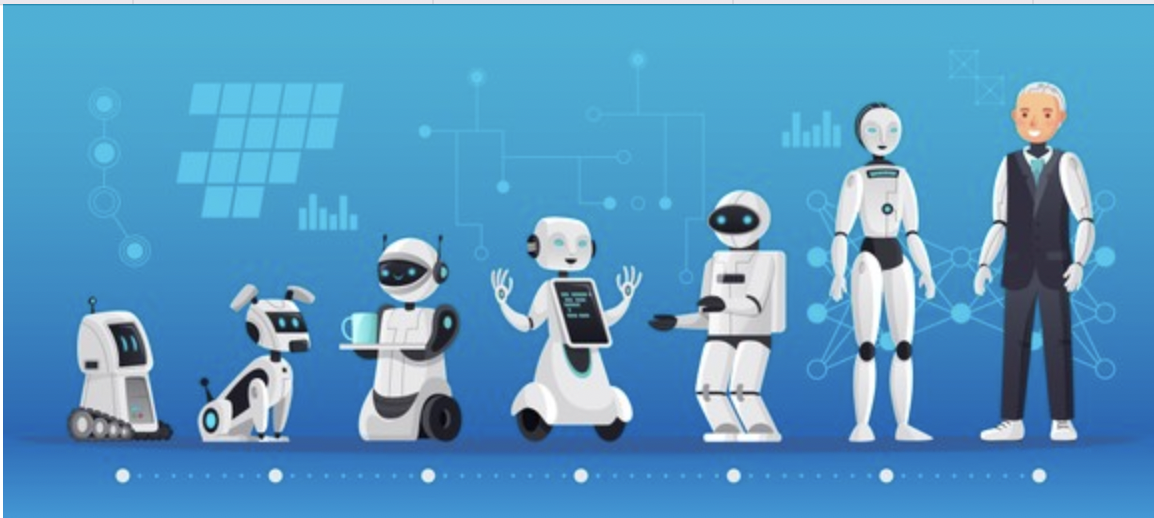
\includegraphics[width=14cm]{assets/Evolution_robots_autonomes.png}
    \caption{Figure montrant l'évolution des robots mobiles autonomes }
    \label{amr}
    \end{figure}

\newpage
Les premiers robots mobiles autonomes (RMA) avaient en fait une autonomie très limitée. Par exemple, les sens et les calculs de Shakey sont encore limités, et planifier une action lui prend des heures. De plus, tout changement dans l'environnement l'obligerait à s'arrêter et à planifier un nouvel évenement . Par exemple, il est impossible de se déplacer en présence d'obstacles mobiles.  

La première méthode proposée pour permettre aux RMA de s'autogérer consiste à "aider" les robots industriels en s'adaptant à leur environnement. Avec le développement de la technologie et de la technologie, les robots "voient" plus et plus vite, "pensent" plus vite, et il devient possible d'explorer moins de travail et moins d'espace fixe. La véritable autonomie des robots offrira de nombreuses perspectives, et dans cet espoir, la robotique mobile autonome devenir une discipline scientifique en soi.

Les robots de service (assistance dans les hôpitaux, les aéroports, les bureaux, les usines ou les habitations), robots de maintenance pour les environnements dangereux ou difficiles d'accès pour l'homme (sous-marin, champs de mines, espace, centrales nucléaires), robots de divertissement (comme celui de Sony récemment sorti de Le Japon des chiens robots et même des véhicules intelligents (voitures autonomes ou systèmes d'assistance) sont quelques exemples d'applications Potentiel des RMA.